\chapter{SẮP XẾP TÔ-PÔ (TOPOLOGICAL SORT)}

\minitoc

\section{Nguồn tài nguyên}

Nội dung bài chủ yếu tham khảo/copy từ [VNOI WIKI] : \url{https://wiki.vnoi.info/algo/graph-theory/topological-sort.md}

\section{Định nghĩa sắp xếp tô-pô}

\begin{dinhnghia}
Cho một đồ thị có hướng \( G = (V, E) \), sắp xếp tô-pô (topological sorting) là một ánh xạ từ tập đỉnh \( V \) vào tập các số nguyên \( \{1, 2, \dots, |V|\} \), sao cho với mọi cung \( (u, v) \in E \), ta có:
\[
\operatorname{order}(u) < \operatorname{order}(v).
\]
\end{dinhnghia}

\begin{dinhnghia}
    Sắp xếp tô-pô là cách sắp xếp các đỉnh của một đồ thị có hướng sao cho nếu có một mũi tên từ đỉnh \( u \) đến đỉnh \( v \), thì \( u \) phải đứng trước \( v \) trong thứ tự đó.
\end{dinhnghia}

Nói cách khác, thứ tự tô-pô là một hoán vị của các đỉnh sao cho mọi cung đều đi từ đỉnh đứng trước đến đỉnh đứng sau trong thứ tự này. Hay nếu một công việc \( u \) cần hoàn thành trước công việc \( v \), thì \( u \) phải xuất hiện trước \( v \) trong danh sách kết quả.



\begin{figure}[H]
    \centering
    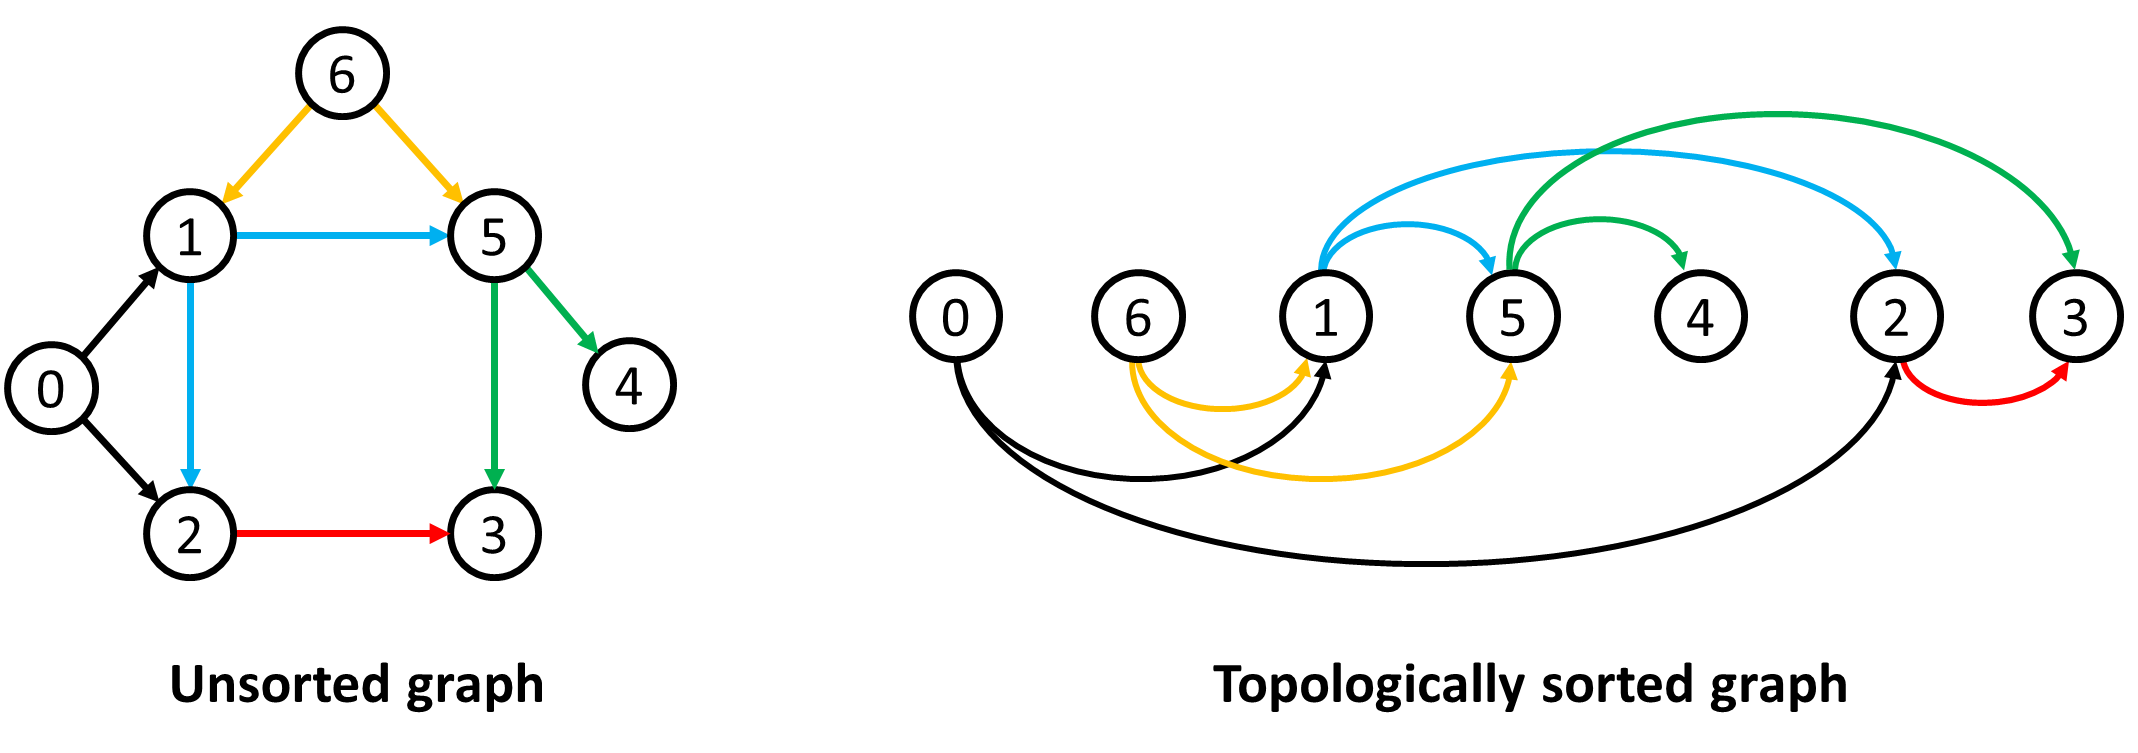
\includegraphics[width=0.6\textwidth]{resource/img/b2/topological_sort_img1.png}
    \caption{Minh họa sắp xếp Tô-pô}
\end{figure}

\section{Cảm hứng và Động cơ ứng dụng}

Sắp xếp tô-pô là một công cụ quan trọng trong việc mô hình hóa và giải quyết các bài toán liên quan đến \textbf{phụ thuộc thứ tự} giữa các đối tượng. Về bản chất, nó cho phép ta xác định một trình tự thực hiện hợp lệ sao cho mọi điều kiện tiên quyết đều được thỏa mãn trước khi thực hiện bước tiếp theo.

Một ứng dụng thực tế điển hình là trong \textbf{lập kế hoạch công việc}. Khi một tập hợp các công việc có quan hệ phụ thuộc lẫn nhau, ta cần xác định thứ tự thực hiện sao cho mỗi công việc chỉ bắt đầu sau khi tất cả các công việc phụ thuộc của nó đã hoàn thành.

\textbf{Ví dụ minh họa:} Trong chương trình đào tạo đại học, sinh viên cần hoàn thành nhiều học phần để tốt nghiệp. Một số học phần là điều kiện tiên quyết cho các học phần khác. Chẳng hạn:
\begin{itemize}
    \item Để học được môn ``Giới thiệu về thuật toán'', sinh viên phải hoàn thành các môn: ``Nhập môn lập trình'', ``Cấu trúc dữ liệu'', ``Nhập môn thuật toán'', v.v.
\end{itemize}

Ta có thể xây dựng một đồ thị có hướng, trong đó:
\begin{itemize}
    \item Mỗi đỉnh tương ứng với một học phần;
    \item Có một cung từ đỉnh \( u \) đến đỉnh \( v \) nếu học phần \( u \) là điều kiện tiên quyết của học phần \( v \).
\end{itemize}

Khi đó, việc tìm một sắp xếp tô-pô của đồ thị này sẽ cho ta một thứ tự học hợp lệ. Nếu không tồn tại sắp xếp tô-pô (tức đồ thị có chu trình), điều đó phản ánh sự xung đột hoặc vòng lặp trong điều kiện tiên quyết giữa các môn học - một cấu trúc bất hợp lệ trong thiết kế chương trình đào tạo.

\begin{ghichu}
Sắp xếp tô-pô không xử lý các xung đột tài nguyên như trùng lịch học, mà chỉ đảm bảo mối quan hệ thứ tự phụ thuộc.
\end{ghichu}


\begin{ghichu}
Chỉ tồn tại sắp xếp tô-pô nếu và chỉ nếu đồ thị là DAG (Directed Acyclic Graph).

\end{ghichu}


\section{Chứng minh điều kiện tồn tại thứ tự Tô-pô}

\begin{giathuyet}
    Một đồ thị có hướng tồn tại thứ tự Tô-pô khi và chỉ khi nó là một \textbf{DAG}.
\end{giathuyet}

\begin{giathuyet}
    Đồng nghĩa, mọi DAG đều tồn tại ít nhất một thứ tự Tô-pô.
\end{giathuyet}

\begin{giathuyet}
    Có thể tìm được một thứ tự Tô-pô bằng thuật toán trong thời gian tuyến tính \( \mathcal{O}(V + E) \).
\end{giathuyet}

\begin{chungminh}
Ta sẽ chứng minh hai chiều của giả thuyết chính.

\textbf{Chiều thuận:} Nếu đồ thị \( G \) có chu trình, thì không thể tồn tại thứ tự tô-pô.

Giả sử tồn tại chu trình \( v_1 \to v_2 \to \dots \to v_n \to v_1 \). Khi đó, theo định nghĩa của thứ tự tô-pô, ta có:
\[
\operatorname{order}(v_1) < \operatorname{order}(v_2) < \dots < \operatorname{order}(v_n) < \operatorname{order}(v_1),
\]
tức là \( \operatorname{order}(v_1) < \operatorname{order}(v_1) \), mâu thuẫn. Vậy, nếu có chu trình, không tồn tại thứ tự tô-pô.\\

\textbf{Chiều nghịch:} Nếu \( G \) là một DAG, thì tồn tại ít nhất một thứ tự tô-pô.

\begin{enumerate}
    \item Vì \( G \) không có chu trình, nên tồn tại ít nhất một đỉnh không có cung đi vào (bậc vào bằng 0). Nếu mọi đỉnh đều có bậc vào \(\geq 1\), thì bắt đầu từ một đỉnh bất kỳ, ta luôn đi được sang đỉnh khác (vì có cung đi vào), và cuối cùng sẽ đi thành một chu trình, mâu thuẫn với giả thiết \( G \) là DAG.

    \item Gọi đỉnh đó là \( u \). Đặt \( u \) là đỉnh đầu tiên trong thứ tự tô-pô.

    \item Loại bỏ \( u \) khỏi đồ thị cùng tất cả các cung đi ra từ \( u \). Đồ thị còn lại vẫn là DAG (vì việc xóa đỉnh không thể tạo ra chu trình mới).

    \item Áp dụng lại quá trình trên với đồ thị còn lại: luôn tồn tại đỉnh có bậc vào bằng 0, đưa nó vào tiếp theo trong thứ tự.

    \item Lặp lại cho đến khi tất cả các đỉnh được đưa vào thứ tự.

    \item Cuối cùng, ta thu được một thứ tự thỏa mãn định nghĩa sắp xếp tô-pô.
\end{enumerate}

\begin{figure}[H]
    \centering
    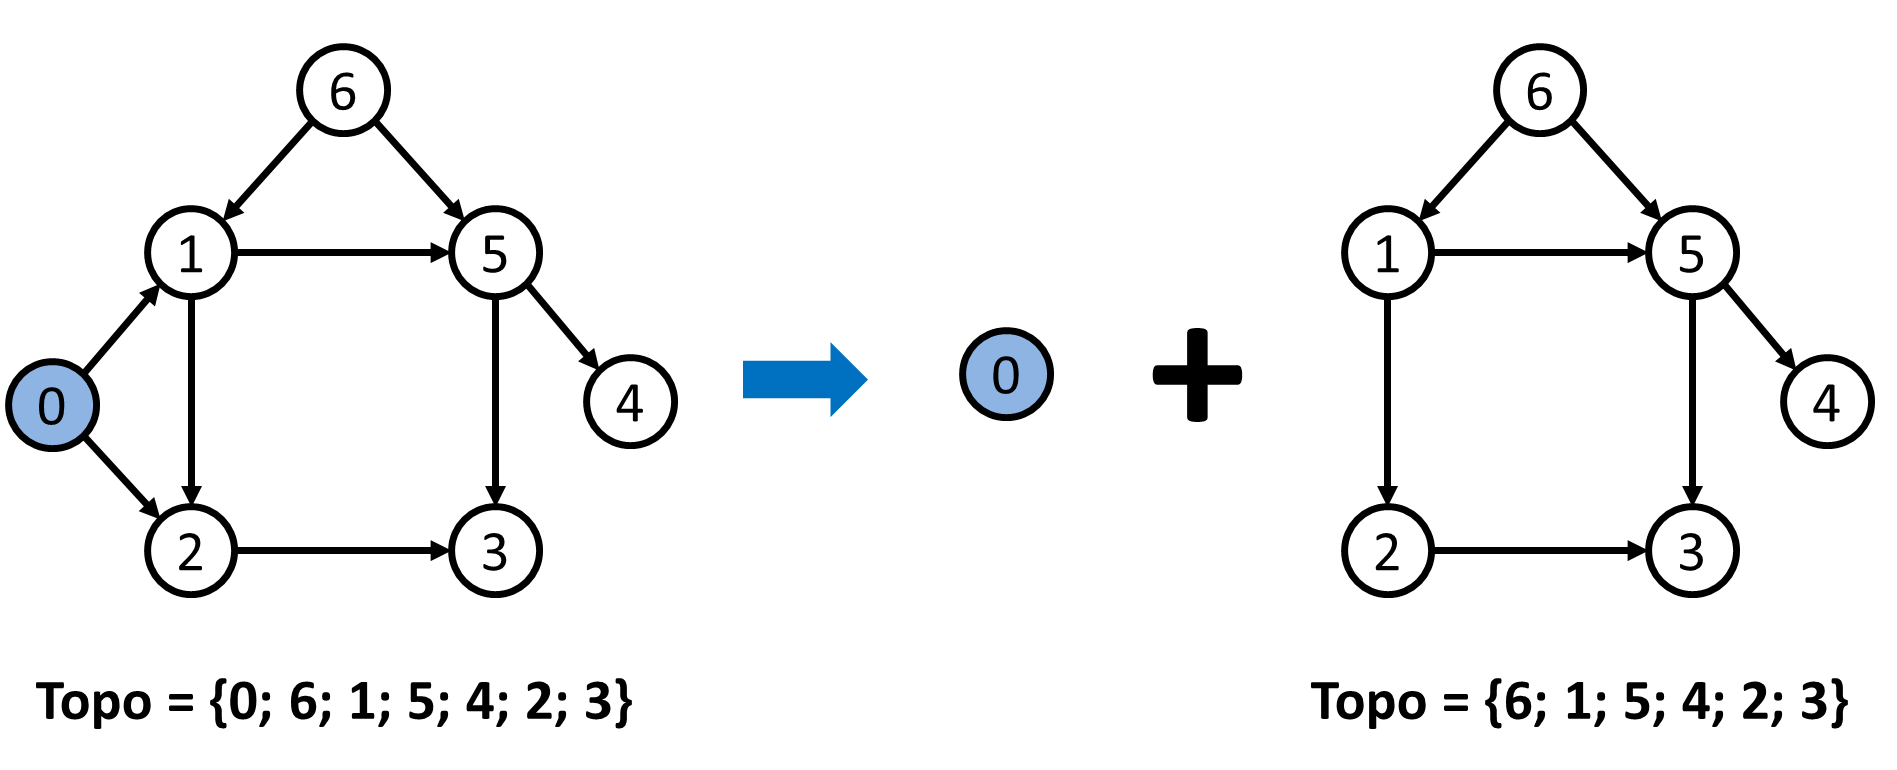
\includegraphics[width=0.6\textwidth]{resource/img/b2/topological_sort_img2.png}
    \caption{Minh họa chứng minh chiều nghịch}
\end{figure}
\textbf{Kết luận:} Với mỗi DAG, luôn tồn tại ít nhất một thứ tự tô-pô.
\end{chungminh}

\section{Bài tập}
\begin{baitap}{TOPOSORT - Sắp xếp TOPO}{}
    
Cho đồ thị có hướng không chu trình $G(V, E)$. Hãy đánh số lại các đỉnh của $G$ sao cho chỉ có cung nối từ đỉnh có chỉ số nhỏ đến đỉnh có chỉ số lớn hơn.

\textbf{Input}

\begin{itemize}
    \item Dòng đầu chứa hai số nguyên $n$ $(1 \leq n \leq 100)$ và $m$ $(0 \leq m \leq \frac{n(n-1)}{2})$
    \item $m$ dòng tiếp theo, mỗi dòng chứa một cặp số $u, v$ cho biết một cung nối từ $u \rightarrow v$ trong $G$.
\end{itemize}

\textbf{Output}

Ghi ra $n$ số nguyên dương, số thứ $i$ là chỉ số của đỉnh $i$ sau khi đánh số lại. Hai số trên cùng một dòng được ghi cách nhau một dấu cách (space).

\textbf{Ví dụ}

\paragraph{Input}
\begin{lstlisting}
7 7
1 2
1 4
2 3
4 5
6 5
5 3
7 4 
\end{lstlisting}

\paragraph{Output}
\begin{lstlisting}
1 2 7 5 6 3 4
\end{lstlisting}

\begin{figure}[H]
    \centering
    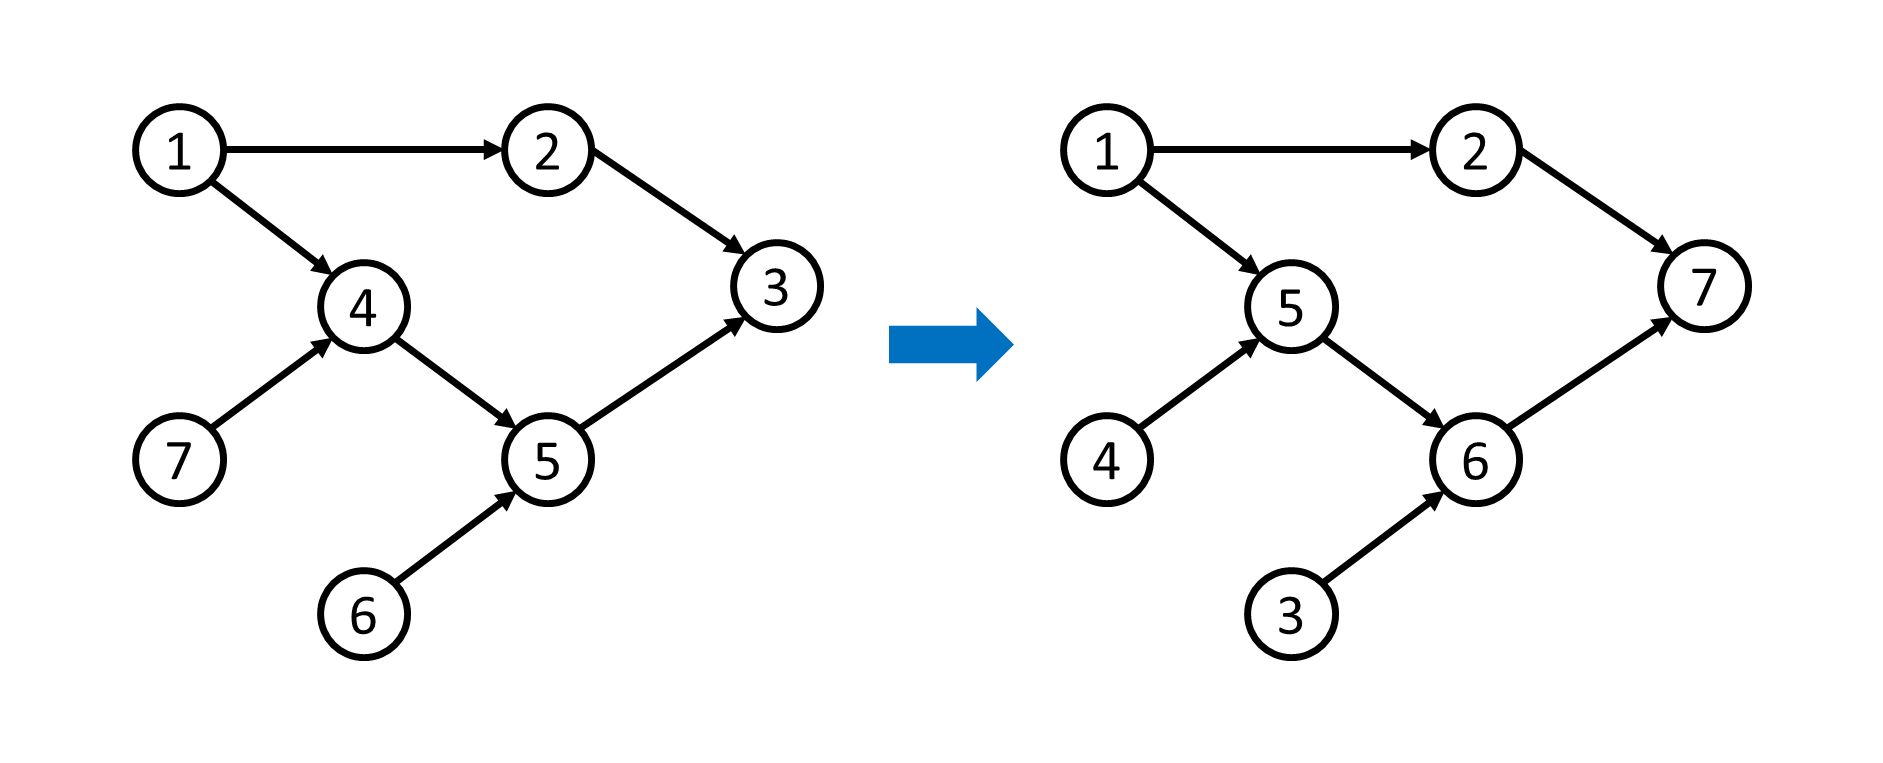
\includegraphics[width=0.6\textwidth]{resource/img/b2/topological_sort_img3.png}
    \caption{Minh họa ví dụ}
\end{figure}

\end{baitap}

\textbf{Phân tích bài toán.}

Với một đỉnh $u$ bất kỳ, khi DFS thăm đến một đỉnh u, sau khi đã đệ quy thăm hết tất cả các đỉnh con của nó, ta đẩy u vào ngăn xếp (\href{https://wiki.vnoi.info/algo/data-structures/Stack}{Stack}). Lúc này ngăn xếp sẽ chứa các đỉnh theo thứ tự ``postorder'' đảo ngược (reverse postorder) -- postorder là thời điểm kết thúc của DFS tại đỉnh đó. 

Để gán nhãn, ta lấy lần lượt từng đỉnh trên cùng của ngăn xếp (tương đương là đỉnh có postorder muộn nhất), gán nhãn lần lượt $1, 2, \dots, n$ đến khi ngăn xếp rỗng (đã xử lý hết đỉnh). Ta đảm bảo được rằng, nếu $u$ được đẩy trước $v$ (tức là hoàn thành DFS sớm hơn), thì $u$ sẽ được gán nhãn lớn hơn.


\paragraph{Cài đặt Sắp xếp Tô-pô bằng DFS}
\begin{lstlisting}[language=C++]
#include <bits/stdc++.h>
#define int long long
#define endl "\n"
using namespace std;

int n, m;
vector<int> adj[101];
stack<int> st;
vector<bool> visited(101, false);

void dfs(int u) {
    visited[u] = true;
    for (auto v : adj[u]) {
        if (visited[v] == false) {
            dfs(v);
        }
    }
    st.push(u);
}

signed main() {
    cin >> n >> m;
    for (int i = 1; i <= m; i++) {
        int u, v; cin >> u >> v;
        adj[u].push_back(v);
    }    
    for (int i = 1; i <= n; i++) {
        if (visited[i] == false) {
            dfs(i);
        }
    }
    vector<int> ans(n + 1, 0);
    int cnt = 1;
    while (st.empty() == false) {
        ans[st.top()] = cnt++;
        st.pop();
    }
    for (int i = 1; i <= n; i++) {
        cout << ans[i] << " ";
    }
    return 0;
}

\end{lstlisting}

\begin{baitap}{Course Schedule}{https://cses.fi/problemset/task/1679}
\noindent
Cho $n$ khóa học, có $m$ yêu cầu có dạng ``khóa học $a$ phải được hoàn thành mới đủ điều kiện học khóa học $b$''. Nhiệm vụ của bạn là tìm thứ tự học sao cho hoàn thành toàn bộ khóa học.

\textbf{Input}

\begin{itemize}
    \item Dòng đầu tiên chứa 2 số nguyên $n$ $(1 \leq n \leq 10^5)$ và $m$ $(1 \leq m \leq 2.10^5)$
    \item $m$ dòng tiếp theo mô tả các yêu cầu. Mỗi dòng chứa hai số nguyên $a$ và $b$ $(1 \leq a, b \leq n)$: khóa học $a$ phải được hoàn thành trước khóa học $b$.
\end{itemize}

\textbf{Output}

In ra thứ tự học để hoàn thành các khóa học. Có thể in bất kỳ thứ tự nào thỏa mãn. 

Nếu không tìm được thứ tự thỏa mãn, in ra ``IMPOSSIBLE''.

\textbf{Ví dụ}

\paragraph{Input}
\begin{lstlisting}
5 3
1 2
3 1
4 5
\end{lstlisting}

\paragraph{Output}
\begin{lstlisting}
4 5 3 1 2
\end{lstlisting}

\end{baitap}



\textbf{Phân tích bài toán.}

Để tìm được thứ tự thỏa mãn, ta phải đảm bảo rằng đồ thị biểu diễn là một DAG. 

Để kiểm tra đồ thị có phải là DAG, ta kiểm tra như sau:
\begin{itemize}
    \item Gọi mảng kiểm tra trạng thái duyệt của đỉnh $i$ bất kỳ là visited[i] = {0, 1, 2} với ý nghĩa lần lượt là: chưa thăm, đang thăm, đã thăm xong.
    \item Khi duyệt đỉnh $u$, đặt trạng thái visited[u] = 1.
    \item Thăm các con $v_i$ của $u$, nếu tồn tại $v_i$ đang có trạng thái visited[$v_i$] = 1, nghĩa là đồ thị có chu trình $\rightarrow$ Không phải là DAG, ta in ra ``IMPOSSIBLE''.
    \item Ngược lại, nếu visited[$v_i$] = 0, ta thăm $v_i$.
    \item Sau khi thăm xong, ta đặt trạng thái visited[u] = 2. 
\end{itemize}

Phần tìm thứ tự là một bài toán Sắp xếp Tô-pô, đã được mô tả thuật toán ở bài \textbf{TOPOSORT - Sắp xếp TOPO} phía trên.

\paragraph{Cài đặt}
\begin{lstlisting}[language=C++]
#include <bits/stdc++.h>
#define int long long
#define endl "\n"
using namespace std;

vector<int> adj[100005];
int n, m; 
vector<int> visited(100005, 0);
stack<int> st;
void dfs(int u) {
    visited[u] = 1;
    for (auto v : adj[u]) {
        if (visited[v] == 1) {
            cout << "IMPOSSIBLE";
            exit(0);
        }
        if (visited[v] == 0) dfs(v);
    }
    visited[u] = 2;
    st.push(u);
}
signed main() {
    cin >> n >> m;
    for (int i = 1; i <= m; i++) {
        int u, v; cin >> u >> v;
        adj[u].push_back(v);
    }    
    for (int i = 1; i <= n; i++) {
        if (visited[i] == 0) {
            dfs(i);
        }
    }
    while (st.empty() == false) {
        cout << st.top() << " ";
        st.pop();
    }
    return 0;
}
\end{lstlisting}


\begin{baitap}{Longest Path}{https://atcoder.jp/contests/dp/tasks/dp\_g}

Cho đồ thị $G$ với $N$ đỉnh và $M$ cạnh. $G$ không tồn tại chu trình có hướng. \\

Hãy tìm độ dài của đường đi có hướng dài nhất trong đồ thị $G$. Độ dài đường đi có hướng dài nhất là tổng số cạnh có trong đường đi đó.

\textbf{Input}

\begin{itemize}
    \item Dòng đầu tiên chứa 2 số nguyên $N$ $(1 \leq n \leq 10^5)$ và $M$ $(1 \leq m \leq 10^5)$
    \item $M$ dòng tiếp theo mô tả các yêu cầu. Mỗi dòng chứa hai số nguyên $x$ và $y$ $(1 \leq x, y \leq n)$ với ý nghĩa: tồn tại cạnh có hướng từ đỉnh $x \rightarrow y$.
\end{itemize}

\textbf{Output}

In ra độ dài đường đi có hướng dài nhất trong đồ thị $G$.

\textbf{Ví dụ}
\paragraph{Input}
\begin{lstlisting}
4 5
1 2
1 3
3 2
2 4
3 4
\end{lstlisting}

\paragraph{Output}
\begin{lstlisting}
3
\end{lstlisting}

\begin{figure}[h]
    \centering
    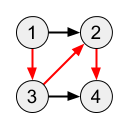
\includegraphics[width=0.1 \textwidth]{resource/img/b2/longest_0_muffet.png}
    \caption{Mô tả ví dụ}    
\end{figure}

\end{baitap}

\textbf{Phân tích bài toán.}

Gọi $dp[u]$ là đường đi có hướng dài nhất kết thúc tại đỉnh $u$. Với $dp[i] = 0, \forall i \in [1..N]$. 

Giả sử đã biết được giá trị $dp[u]$, với mỗi cạnh có hướng từ $u \rightarrow v$, ta cập nhật được:
\[
    dp[v] = \max(dp[v], dp[u] + 1)
\]

Với ý nghĩa là nếu ta đi từ $u \rightarrow v$, thì đường đi có hướng dài nhất kết thúc ở $v$ có thể thu được bằng đường đi có hướng dài nhất đến $u$ cộng thêm 1 bước.

Để đảm bảo mỗi khi cập nhật dp[v] thì dp[u] đã được tính xong, ta duyệt các đỉnh theo thứ tự tô-pô của đồ thị.\\

Như vậy, sau khi lặp qua hết các cạnh theo thứ tự tô-pô, giá trị $\max_{1 \leq i \leq N} dp[i]$ chính là độ dài đường đi có hướng dài nhất trong toàn đồ thị.\\

\textbf{[Groot]:} Ê khoan, tao thắc mắc là tại sao với $dp[v]$ cần lấy $\max(dp[v], dp[u] + 1)$?\\

\textbf{[vuivethoima]:} Mày có thật sự từng đạt giải 3 OLP'24 không vậy? Tao nghi ngờ cái giải của mày rồi đó. Thôi để tao nói luôn, vì trước khi thăm $v$ từ đỉnh $u$, có thể tồn tại đường đi dài nhất kết thúc tại $v$ mà không thông qua đỉnh $u$. Vì vậy ta cần lấy $\max$ của 2 trường hợp: tồn tại đường đi dài nhất kết thúc tại $v$ mà: không qua $u$ $\&$ qua $u$.\\

\textbf{[vuivethoima]:} Mà code tới đây tao lười xử lý/thao tác trên ngăn xếp (stack) nên sau này với các bài toán sắp xếp tô-pô, tao sẽ thao tác trên vector và reverse vector để lấy thứ tự tô-pô (Vector is the best data structure in C++/the world).

\paragraph{Cài đặt}
\begin{lstlisting}[language=C++]
#include <bits/stdc++.h>
#define int long long
#define endl "\n"
using namespace std;

vector<int> adj[100005];
int n, m; 
vector<int> visited(100005, 0);
vector<int> dp(100005, 0);
vector<int> st;

void dfs(int u) {
    visited[u] = true;
    for (auto v : adj[u]) {
        if (!visited[v]) dfs(v);
    }
    st.push_back(u);
}

signed main() {
    cin >> n >> m;
    for (int i = 1; i <= m; i++) {
        int u, v; cin >> u >> v;
        adj[u].push_back(v);
    }    

    for (int i = 1; i <= n; i++) {
        if (visited[i] == false) {
            dfs(i);
        }
    }
    reverse(st.begin(), st.end());

    for (auto u : st) {
        for (auto v : adj[u]) {
            dp[v] = dp[u] + 1;
        }
    }
    int ans = 0;
    for (int i = 1; i <= n; i++) ans = max(ans, dp[i]);
    cout << ans;
    return 0;
}
\end{lstlisting}